%Author: Marius
\paragraph{Motivation}
While sophisticated algorithms like the random cut forest seem to be promising for fitting large amounts of data with complex patterns, they did appear overly complicated for the amount and nature of the data at hand. Apart from holidays, the data shows a clear weekly periodicity, where the data from one week can hardly be distinguished from another. In fact, the weeks are so similar, that we can predict the same pattern every week with high confidence. This motivated us to implement a very simple, yet effective machine learning model called the Mean Predictor.

\paragraph{Idea}
Unsurprisingly, the name says it all. The objective of the Mean Predictor is to calculate the expected week and standard deviation for each point in a week. Accordingly, we can identify outliers by simply checking if the data point lies within the allowed deviation of the expected value. 

Unfortunately, AWS Sagemaker does not offer a Mean Predictor as an Out-Of-The-Box algorithm like the Random Cut Forest. Thus, we implemented it by ourselves.

\paragraph{Implementation}

\begin{figure}
    \centering
    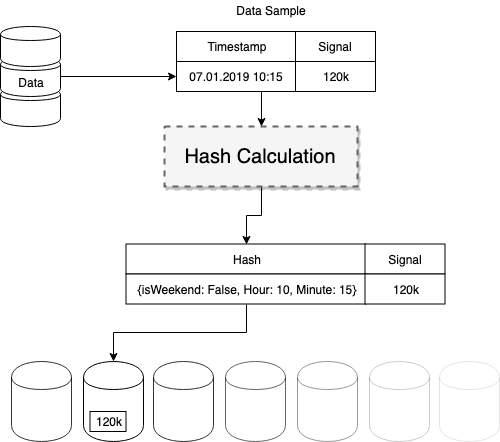
\includegraphics[width=0.6\textwidth]{images/mean_predictor_hashing.png}
    \caption{Hashing process of Mean Predictor Model}
    \label{fig:mean_predictor_hashing}
\end{figure}

For calculating the expected week, we sorted every data point into a bucket that is determined by its timestamp. Each bucket has a hash or index associated with them. After distributing all the data into buckets, we calculate the mean of all the values in one bucket, as well as a measure of standard deviation. This process is visualized in figure \ref{fig:mean_predictor_hashing}.

The hashing function is central to this approach, as we can arbitrarily craft the features that we want our mean predictor to represent. Apart from the weekly periodicity of the data, we also noticed a very predictable daily pattern throughout the working week. Hence we decided to put all working days into one set of buckets, while we put all weekend days into another. We did this to ensure a reasonable amount of samples for each bucket. The hashing function currently employed in the mean predictor is shown in  code example \ref{lst:timestamp_hashing} shows the hashing function employed in our solution. As more and more data comes in, the function can be adjusted to one's needs.

% wrap in minipage so the code doesnt get split to multiple pages
\begin{minipage}{\linewidth}
\begin{lstlisting}[caption={Time stamp hashing function used for Mean Predictor},label={lst:timestamp_hashing}]
def __time_hash(self,t):
       return (t.weekday() < 5,t.hour,t.minute)

\end{lstlisting}
\end{minipage}

As mentioned before, we also require a measure of expectation deviation for determining outliers. What first comes to mind is the standard deviation:

\begin{equation}
\begin{aligned}
\sigma_t = \sqrt{\frac{1}{n}\sum_{i=1}^N (s_t^{(i)} - \mu_t)^2}\\
\end{aligned}
\end{equation}

Where $\mu_t$ denotes the mean value of bucket $t$ and $s_t^{(i)}$ the $i$-th value in this bucket. However, since we square the distance from the mean, the standard deviation weighs outliers much heavier than conform data, which might not be the desired behaviour for the task at hand, because outliers are what we want to detect. Instead one might want to use the average euclidean distance from the mean:
\begin{equation}
\begin{aligned}
\sigma_t = \frac{1}{n}\sum_{i=1}^N \sqrt{(s_t^{(i)} - \mu_t)^2}\
\end{aligned}
\end{equation}
In our case, the choice of deviation measure had little influence on the final results, nevertheless if future training data is noisy and contains a lot of outliers, this might be an option to consider. 

\paragraph{Training and Prediction}
\begin{figure}[h]
    \centering
    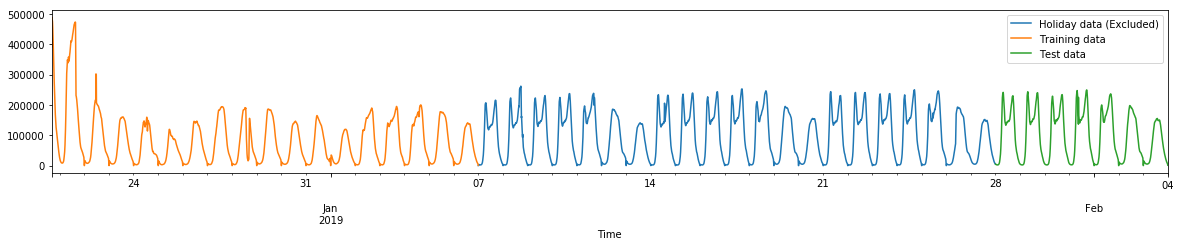
\includegraphics[width=1\textwidth]{images/mean_pred_training_data.png}
    \caption{Train-Test split of data used for the mean predictor}
    \label{fig:mean_predictor_training_data}
\end{figure}
Due to Christmas holiday, a lot of the provided training data is anomalous, thus not useful for training a model that is supposed to detect anomalies. Accordingly, we excluded this data from training, leaving us with only three weeks of training data. Alternatively one could also alter the hashing function to give holidays a separate set of buckets. Our train-test split is shown in figure \ref{fig:mean_predictor_training_data}

\begin{figure}
    \centering
    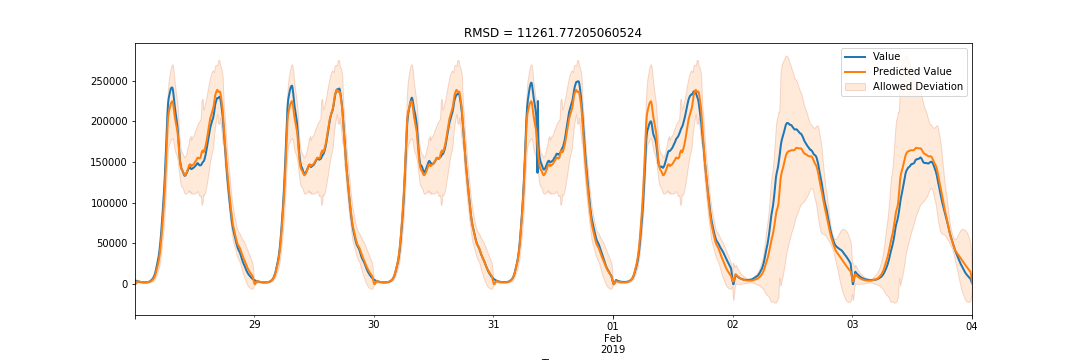
\includegraphics[width=1\textwidth]{images/mean_pred_test.png}
    \caption{One week prediction of mean predictor model}
    \label{fig:mean_predictor_prediction}
\end{figure}

Once we have expected value and deviation for each bucket, making predictions is trivial. For prediction, the model simply takes a timestamp interval and calculates the hash for each one. We obtain the prediction by simply looking up the expected value and deviation in our table. Figure \ref{fig:mean_predictor_prediction} depicts a prediction for the week starting at the 28th of January 2019 and compares it to the ground truth. For this test data, the prediction is highly accurate and the true values never leave the confidence interval. Since we lack real testing data that can be used to assess the outlier detection performance, we must leave it at the intuition that what is outside of the confidence interval is considered anomalous. The RMSE of the prediction lies around 11,261.
\pagebreak

\paragraph{Deployment as Sagemaker Endpoint}
In order to use our model in the Cloud, we had to deploy it as an AWS Sagemaker Endpoint. In the following we describe the technical details related to this task. The endpoint was implemented along the lines of a tutorial provided by AWS \footnote{\url{https://github.com/awslabs/amazon-sagemaker-examples/blob/master/advanced_functionality/scikit_bring_your_own/scikit_bring_your_own.ipynb}}.

Sagemaker Models are deployed from docker images. Hence, we defined a docker file that encapsulates the model into a container. The container image is then built uploaded to AWS \textit{Elastic Container Registry} (ECR) with the \textit{build\_and\_push.sh} script. The \textit{train\_deploy.py} script provides a convenient commandline interface for spinning up a Sagemaker endpoint using the previously uploaded container image. This script can also be embedded into a terraform pipeline.
The model requires only one hyperparameter: The granularity or \textit{frequency} with which it should make the time series predictions. Furthermore it needs a path to the training data located in a S3 Bucket.

At its core, the Sagemaker endpoint is nothing but a REST-API that takes training jobs and prediction requests and forwards it to the Mean Predictor. Once deployed, the endpoint takes prediction requests in the following JSON format:

\begin{lstlisting}
{
    "start": "YYYY-MM-DD HH:MM:00",
    "end": YYYY-MM-DD HH:MM:00
}
\end{lstlisting}

It will respond with a time series prediction within the \textit{start}-\textit{end} interval, depending on the aforementioned \textit{frequency}. The response is delivered in the following CSV-Format:

\begin{center}
    \begin{tabular}{ | l | l | l |}
    \hline
    Timestamp & Value & Std \\ \hline
    2019-01-05 10:15:00 & 100 & 7 \\ \hline
    2019-01-05 10:20:00 & 96 & 13 \\ \hline
    2019-01-05 10:25:00 & 112 & 8 \\ \hline
    \dots & \dots & \dots \\
    \hline
    \end{tabular}
\end{center}

Similar to the Random Cut Forest, the model will not do outlier detection by itself, but rather provide the user with the necessary information to do so. In order to detect an outlier, one must simply check if a specific data point lies within the bounds of allowed deviation at that time. The user can arbitrarily scale the allowed deviation to their requirements. Such functionality is easily implemented within an AWS Lambda function, which allows seamless integration of the model into the Cloud Architecture. Furthermore, it allows to use the same model for anomaly detection and prediction at the same time.

\paragraph{Conclusion}
The Mean Predictor is of course a very minimalistic approach: In its current state, we can only incorporate a single source of information, it is not able to leverage additional data, e.g. weather data to improve its prediction. The model is not able to learn features of the time series by itself. As the prediction will resemble a regular working week every time, the model is of little use during holiday periods, however, once enough data is gathered, the hashing function can be manually adjusted to differentiate between holiday and working weeks. With the  small amounts of training data we have and the selected test set, the prediction of the Mean Predictor vastly outperforms the other, more complex, Machine Learning models that we examined with an RMSE of just 11,261.